\documentclass[11pt]{article}
\usepackage{latexsym}
\usepackage{amsmath}
\usepackage{amssymb}
\usepackage{amsthm}
\usepackage{epsfig}
\usepackage[tight]{subfigure}

\usepackage{amsmath}

\DeclareMathOperator*{\minimize}{min}
\DeclareMathOperator*{\maximize}{max}

\usepackage{algorithm}
 %on linux you may need to run sudo apt-get install texlive-full to install algorithm.sys
\usepackage{algorithmic}

\usepackage{verbatim}

\newcommand{\handout}[5]{
  \noindent
  \begin{center}
  \framebox{
    \vbox{
      \hbox to 5.78in { {#1} \hfill #2 }
      \vspace{4mm}
      \hbox to 5.78in { {\Large \hfill #5  \hfill} }
      \vspace{2mm}
      \hbox to 5.78in { {\em #3 \hfill #4} }
    }
  }
  \end{center}
  \vspace*{4mm}
}

\newcommand{\lecture}[5]{\handout{#1}{#2}{#3}{#4}{#5}}
\newcommand{\collision}[0]{\mathrm{collision}}
\newcommand{\nocollision}[0]{\overline{\collision}}

\newcommand*{\QED}{\hfill\ensuremath{\square}}

\newtheorem{theorem}{Theorem}
\newtheorem{corollary}[theorem]{Corollary}
\newtheorem{lemma}[theorem]{Lemma}
\newtheorem{observation}[theorem]{Observation}
\newtheorem{proposition}[theorem]{Proposition}
\newtheorem{definition}[theorem]{Definition}
\newtheorem{claim}[theorem]{Claim}
\newtheorem{fact}[theorem]{Fact}
\newtheorem{assumption}[theorem]{Assumption}
\newtheorem{note}[theorem]{Note}

% 1-inch margins, from fullpage.sty by H.Partl, Version 2, Dec. 15, 1988.
\topmargin 0pt
\advance \topmargin by -\headheight
\advance \topmargin by -\headsep
\textheight 8.9in
\oddsidemargin 0pt
\evensidemargin \oddsidemargin
\marginparwidth 0.5in
\textwidth 6.5in

\parindent 0in
\parskip 1.5ex
%\renewcommand{\baselinestretch}{1.25}

\begin{document}

\lecture{Statistical Techniques in Robotics (16-831, S20)}{Lecture \#22
  (Monday, April 26)}{Lecturer: Kris Kitani}{Scribes: Zhekai Jin}{Imitation Learning \& LP-IRL}

\section{Review}
In the last few lectures, We spent a lot of time going over the key algorithms in the field of Reinforcement Learning(RL). As you may recall in the Littman Nature Graph \cite{littman2015reinforcement}, RL algorithms lies in the field of sampled, evaluative and sequential feedback as a Sequential Decision-Making algorithm. There are many RL approaches to find the optimal policy and we analyzed three main types of RL algorithms: (1) Policy-based, (2) Hybird, and (3) Value-based. And with different assumptions on finding the optimal policy, RL algorithms loosely divide into (1) Model-based and (2) Model-free algorithms. We went over some mainstream algorithms for Model-based RL: (1) value iteration, and (2) policy iteration and some for Model-free RL: (1) Temporal Differencing, (2) Policy gradient, (3) Actor-Critic. And We covered the last two specifically in the last lecture. In this lecture, we will introduce and analyze the field of Imitation Learning (IL) and motivates the invention of IL. And We will learn a specific type of IL algorithm: Inverse Reinforcement Learning (IRL) algorithm. A quick gist for understanding the motivation of the invention of IL could be interpreted as using expert advice/demo to guide the algorithm to quickly navigate through the typical humongous state spaces of RL learning  for faster learning speed and model/learn the reward function to generalize the algorithm enough for variation of the environment (which often assumed to be static for RL algorithms). This lecture, after the review section, will motivates and introduce the Imitation Learning field and formulate the Linear Programming - IRL problem. In the next two subsections, we will first recap the problem of RL and a few definitions to help us along the way in understanding IL. 

%This section serves as a review of the previous lecture and any other context required to frame the content of the current lecture. 

%You may format the scribes in any way you like, aside from changing font style, size and page format. Please use subsections and paragraphs to increase the readability of your notes.

%Length requirement 1-2 pages.
        
\subsection{Reinforcement Learning}
Reinforcement Learning could be generalized as the problem of an agent tying to learn an optimal, or nearly-optimal, policy that maximizes the "reward function" or other user-provided reinforcement signal that accumulates from the immediate rewards. Theoretically, we often map the RL environment to a Markov Decision Process(MDP) description to guarantees the theoretical result as MDP presents the Bellman Equation as a recursive relationship between value functions for a useful constraint for optimization. We could formulate a Markov Decision Process (MDP) as $(\mathcal{S}, \mathcal{A}, P, r, H, \rho)$, where $\mathcal{S}$ is the state space, $\mathcal{A}$ is the action space, $P$ is the transition dynamics such that $P\left(s^{\prime} \mid s, a\right)$ is the probability of reaching state $s^{\prime}$ from $s$ by taking action $a ; r(s, a)$ is the reward of taking action $a$ at state $s$ and $H$ is the planning horizon; $\rho$ is the initial distribution where we sample the initial state $s_{1} .$ We cloud then define policy $\pi: \mathcal{S} \rightarrow \Delta(|\mathcal{A}|)$, namely $\pi(a \mid s)$ is the probability of $\pi$ taking action $a$ at state $s$. Given the MDP and a policy $\pi$, we could define any trajectory as $\tau=\left\{s_{1}, a_{1}, s_{2}, a_{2}, \ldots, s_{H}, a_{H}, s_{H+1}\right\}$, where $s_{1} \sim \rho, a_{t} \sim \pi\left(\cdot \mid s_{t}\right)$ and $s_{t+1} \sim P\left(\cdot \mid s_{t}, a_{t}\right) .$ and define the total reward of such trajectory as $R(\tau)=$ $\sum_{t=1}^{H} r\left(s_{t}, a_{t}\right)$. Mathematically, the RL algorithm tries to maximize the expected total reward of a trajectory from start state until the planning horizon is reached.

\subsection{Types of RL algorithms}
We recall that RL algorithms could be classified into three types:
\begin{enumerate}
    \item Value-Based: these type of algorithms learn the state or state-action value. Act by choosing the best action in the state. Exploration is necessary. 
    \item Policy-Based: learn directly the stochastic policy function that maps state to action. Act by sampling policy.
    \item Hybrid: a mix of above 
\end{enumerate}
Note that in Policy-based methods we explicitly build a representation of a policy (mapping $\pi: s \rightarrow a)$ and keep it in memory during learning. However, in Value-based we don't store any explicit policy, only a value function. The policy is here implicit and can be derived directly from the value function (pick the action with the best value).

Note on previous lecture we also discussed an extension on this classifying RL algorithms based on On-policy vs. Off Policy: This division is based on whether you update your $Q$ values based on actions undertaken according to your current policy or not. 

\subsection{Assumptions of RL algorithms}

As we mentioned in the introduction, we could again divide RL algorithms based on their underlying assumptions :
\begin{enumerate}
    \item Model-Based: The algorithm has full access to the environment including state transition dynamics and reward function.
    \item Model-Free: only samples could be drawn from the environment.
\end{enumerate}

As we can see, Model-based methods (value or policy iteration as we discussed) use the model of the environment, which is usually represented as a Markov decision process. More specifically, the model consists of the transition and reward functions of the Markov decision process, which should represent the dynamics of the environment. As in policy iteration, the rewards (used to estimate the policy or value functions) are not the result of the interaction with the environment but directly given by the MDP (the model of the environment), so the decisions are made according to the reward function (and the transition function) of the MDP that represents the dynamics of the environment. And we could fully write out the state expansion in the derivation in earlier lectures. Model-based methods usually are not dependent on past actions, as we see policy iteration converges to the optimal policy independently of the initial values of the states, the initial policy or the order of iteration through the states.

Model-free methods, such as Monte Carlo methods do not use such a model, even though the assumption that the environment can be represented as an MDP is often implicitly made. In the case of Monte Carlo methods, all estimates are solely based on the interaction with the environment (with samples drawn). In general, Monte Carlo methods are based on sampling (or random) operations. The samples are the rewards that are obtained when certain actions are taken from certain states.

\section{Summary}
\subsection{Imitation Learning}
\subsubsection{Motivation for Imitation Learning}
As we have seen, Reinforcement learning (RL) is one of the most interesting areas of machine learning, where an agent interacts with an environment by following a policy. In each state of the environment, it takes action based on the policy, and as a result, receives a reward and transitions to a new state. The goal of RL is to learn an optimal policy which maximizes the long-term cumulative rewards. To achieve the reward maximization, RL is also trying to solve a few problem: the exploration-exploitation trade-off, the problem of delayed reward (credit assignment), and the need to generalize.
Generally, RL methods perform really well by using the received rewards as the main approach to approximate the best policy. However, in some cases, though the teaching process is challenging. This can be especially true in an environment where the rewards are sparse (e.g. a game where we only receive a reward when the game is won or lost). To help with this issue, we can manually design rewards functions, which provide the agent with more frequent rewards. Also, in certain scenarios, there isn’t any direct reward function (e.g. teaching a self-driving vehicle), thus, the manual approach is necessary. However, manually designing a reward function that satisfies the desired behaviour can be extremely complicated, as the reward function for the MDP setting is often hard to define and taking months to tune with a usually large amount of state variables.
A feasible solution to this problem is imitation learning (IL). In IL instead of trying to learn from the sparse rewards or manually specifying a reward function, an expert (typically a human) provides us with a set of demonstrations. The agent then tries to learn the optimal policy by following, imitating the expert’s decisions.

\subsubsection{Problem Formulation}
\normalfont
We first present a few definition to define the Imitation Learning(IL) problem. The IL problem could be formally defined as 
$$
\mathcal{A}_{\mathrm{IL}}:\left\langle\mathcal{D}^{*}, \pi^{*}, \mathcal{T}, \mathcal{R}\right\rangle \rightarrow \pi
$$
And the equation could be broken down as 

\begin{enumerate}
    \item Expert demonstrations: 
    $$
\mathcal{D}^{*}=\left\{\boldsymbol{\zeta}_{n}\right\}_{n=1}^{N} \sim \mathcal{E} \mid \pi^{*}
$$
    Expert demonstrations are defined as a set of exemplary trajectories sampled from the optimal policy $\pi^{*}$. The representation form of demonstrations is flexible though, as it could be represeted either as 
    $$\text{state sequence}\quad \boldsymbol{\zeta}=\left\{s^{(0)}, s^{(1)}, \ldots, s^{(T)}\right\}$$  
    or 
    $$\text{a sequence of state-action pairs}\boldsymbol{\zeta}=\left\{s^{(0)}, a^{(0)}, s^{(1)}, \ldots, a^{(T-1)}, s^{(T)}\right\}$$
    \item Optimal policy(Oracle): 
    $$
    \pi^{*}(a \mid s)
    $$
    Optimal policy is the expert policy where the expert demonstrations are sampled from. As you may wonder why we could not just copy from the optimal policy and get the job done.
    It should be noted that the optimal policy may not be always be available to the agent and the policy could be sub-optimal in a sense that it may not be general enough for a variable/similar environment. Also, even if accessible, the optimal policy will be given to the agent as samples without full parameterization, making IL a nontrivial task.
    
    \item Dynamics function and Reward function: 
    $$
    P\left(s^{\prime} \mid s, a\right), R\left(s, a\right)
    $$
    The main component of IL is the environment, which is still, essentially a Markov Decision Process (MDP). This means that the environment has an $S$ set of states, an $A$ set of actions, a $P(s’|s,a)$ transition model (which is the probability that an action a in the state s leads to state s’ ) and an $R(s,a)$ reward function. However the transition model and reward function could be sampled from the environment, however may not always be available to the agent as we will see in the next section.
\end{enumerate}

\subsubsection{A Classification on IL Algorithms}
\begin{table}[h]
\centering
\begin{tabular}{|c|c|c|c|}
\hline
Var/type        & Passive IL & Active IL & Interactive IL \\ \hline
Demonstrations $D^*$     & yes        & yes       & optional       \\ \hline
Environment $\varepsilon$ & no         & yes       & yes            \\ \hline
Oracle $\pi^*$           & no         & no        & yes            \\ \hline
Dynamics $T$             & no         & optional  & optional       \\ \hline
Reward $R$               & no         & optional  & optional       \\ \hline
\end{tabular}
\caption{ A Classification on IL Algorithms}
\label{tab:IL-type}
\end{table}

With these four definitions may or may not be available to the agent, the IL algorithms could be divide into three categories. 

\begin{enumerate}
    \item Passive IL: Passive IL, also known as behavior cloning, focuses on learning the expert’s policy using supervised learning. An important example of behaviour cloning is ALVINN, a vehicle equipped with sensors, which learned to map the sensor inputs into steering angles and drive autonomously. This project was carried out in 1989 by Dean Pomerleau, and it was also the first application of imitation learning in general.
    The way behavioural cloning works is quite simple. Given the expert’s demonstrations, we divide these into state-action pairs, we treat these pairs as i.i.d. examples and finally, we apply supervised learning. The loss function can depend on the application. As we could see from Table \ref{tab:IL-type}, only expert demonstrations are available to the agent and the algorithm does not interacts with the environment at all. It lies with online linear classification algorithms with sampled one-shot feedback in the Littman Nature Graph shown in Figure \ref{fig:lion}.
    \item Active IL:
    Active IL get expert demonstration and access to the environment, but does not have access to the optimal policy. Optionally, It interacts with the environment with drawing samples upon the reward and state transition dynamics. As we are going to discuss the Inverse Reinforcement Learning, which is a type of Active IL. It lies just as RL algorithm in the 
    Littman Nature Graph shown in Figure \ref{fig:lion}.
    
    \item Interactive IL:
    Interactive has all other access to the environment, making the expert demonstrations optional to the agent as it has access to the oracle policy, serving as an alternative of expert demonstrations. As we might observe, Interactive IL perceives sequential instructive feedback from the environment, which could not be represented well in the Littman Nature Graph shown in Figure \ref{fig:lion} \cite{littman2015reinforcement}.
     
\end{enumerate}

\begin{figure}[H]
\centering
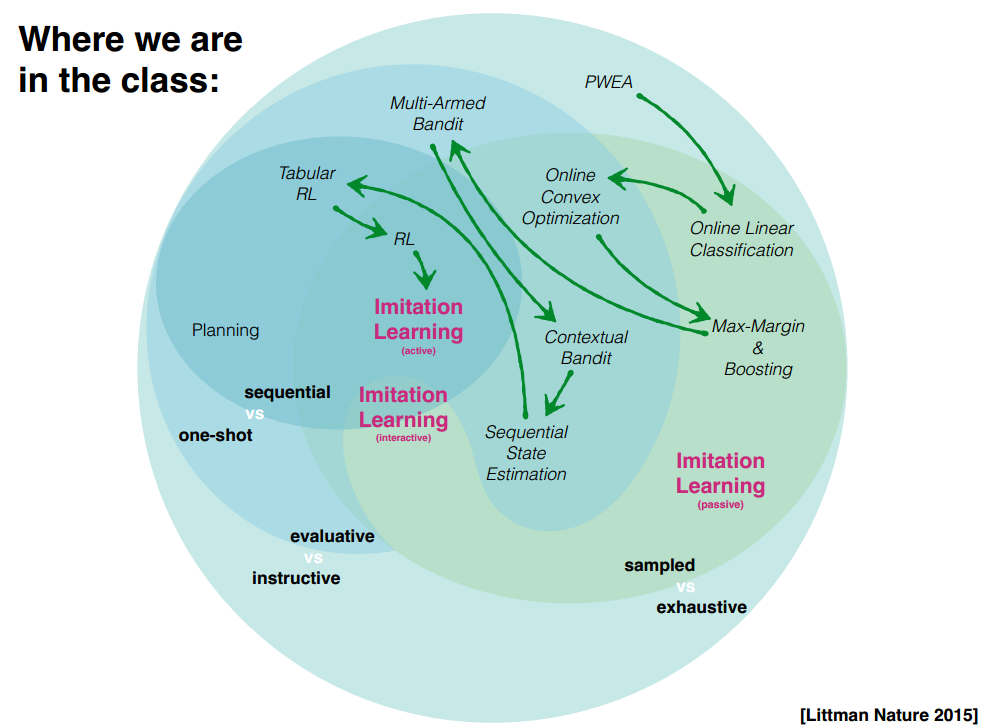
\includegraphics[width=0.8\linewidth]{1.png}
\caption{Littman Nature Graph}
\label{fig:lion}
\end{figure}


\subsection{Linear Programming - Inverse Reinforcement Learning}
\subsubsection{Motivation}
Inverse Reinforcement Learning is a type of Active IL, which is the field of learning an agent’s objectives, values, or rewards by observing its behavior. The algorithms is trying to not only estimate the optimal policy but also learn the reward function to get better understanding of the environment/task. The reward function, which could be hard to define for an RL problem, could be learned in IRL and feed into the RL framework to learn an optimal policy, as shown in Figure \ref{fig:IRL}. Moreover, a reward function learned this way might be more general to fit environment similar to the training environment.

\begin{figure}[H]
\centering
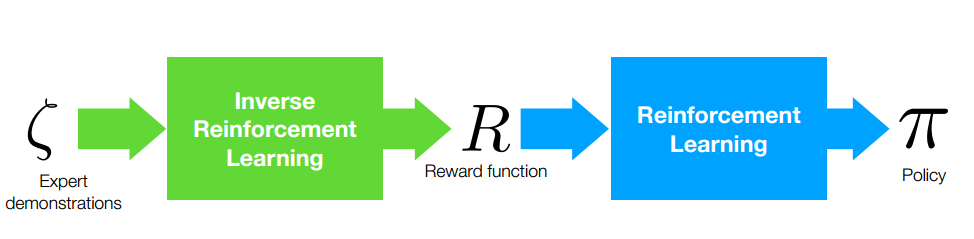
\includegraphics[width=0.8\linewidth]{2.png}
\caption{Inverse Reinforcement Learning Paradigm}
\label{fig:IRL}
\end{figure}

\subsubsection{Algorithms for  Inverse Reinforcement Learning}
The invention of IRL could be traced back at this work by Andrew, N.G.\cite{ng2000algorithms},
where three algorithms of IRL are given:
\begin{enumerate}
    \item IRL for finite state spaces
    \item IRL for large state spaces
    \item IRL from sampled trajectories
\end{enumerate}
Note all the algorithms here are solved by tackling a linear programming problem, And the paper\cite{ng2000algorithms} steps through the IRL problem with order present above. We are going to review them in the same order in this and the following lectures.

\subsubsection{Inverse Reinforcement Learning for finite spaces}
Firstly, we define the goal of this algorithm to be: \\
\textbf{Goal:} Find the reward function(s) such that the policy is optimal.\\ 
And for this algorithm, we have a few strict and often unpractical assumptions: \\
\textbf{Assumptions}:
\begin{itemize}
    \item State space is finite.
    \item Transition model is known.
    \item Complete policy is known.
\end{itemize}
As we often observe in real world problems, the state space is often continuous, the transition model may not be accessible from the environment as it is present optional in the active-IL setting, and the optimal policy may not be accessible as well. 

To solve such an optimization problem, we firstly need to define an objective function: \\
\textbf{Objective function:} Find the reward function(s) such that the policy is optimal.\\ 
$$
\max _{R}\left\{\sum_{s} Q^{\pi}\left(s, a^{*}\right)-\max _{a \neq a^{*}} Q^{\pi}(s, a)\right\}
$$
The objective function of IRL-finte space is trying to maximize the reward, as RL problems do.
It could be interpreted as trying to maximize the difference between the cumulative reward of the optimal policy and the second best policy, which in turn find the best optimal policy that has largest difference over all other policies. Recall that the Q value is related to the reward as we covered in previous lectures as $Q^{\pi}(s, a)=R(s)+\gamma \sum p\left(s^{\prime} \mid s, a\right) V^{\pi}\left(s^{\prime}\right)$.

This objective function is a linear programming problem. However, this objective function is not easy to optimize as the $Q$ function is unbounded and the first term could goes to infinity with second term goes to negative infinity to have the optimal results. We add an regularization term to add an bound to the reward function as the bigger the reward values are , the more we get penalized. Thus the final objective function:
$$
\max _{R}\left\{\sum_{s} Q^{\pi}\left(s, a^{*}\right)-\max _{a \neq a^{*}} Q^{\pi}(s, a)\right\}-\lambda\|R\|_{1}
$$

To make the linear programming part more obvious, we reveal this problem in matrix form:
Recall the definition of Q value function:
$$
Q^{\pi}(s, a)=R(s)+\gamma \sum_{s^{\prime}} p\left(s^{\prime} \mid s, a\right) V^{\pi}\left(s^{\prime}\right) \quad \forall s, a
$$
We could rewrite it in matrix form as:
$$
\mathbf{Q}^{\pi}(a)=\left(\mathbf{R}+\gamma \mathbf{P}_{a} \mathbf{V}^{\pi}\right) \quad \forall a
$$
where all equations for some action a is presented as a matrix form.\\

Like wise, we present the V function in matrix form from:
$$
V^{\pi}(s)=R(s)+\gamma \sum_{s^{\prime}} p\left(s^{\prime} \mid s, a=\pi(s)\right) V^{\pi}\left(s^{\prime}\right) \quad \forall s
$$
to:
$$
\begin{aligned}
\mathbf{V}^{\pi} &=\left(\mathbf{R}+\gamma \mathbf{P}_{a} \mathbf{V}^{\pi}\right) \\
 &=\left(\mathbf{I}-\gamma \mathbf{P}_{a}\right)^{-1} \mathbf{R}
\end{aligned}
$$
As we could observe, with finite state space and known expert policy, we could do policy iteration with dynamic programming, though this constraints not often practical. To keep going, we could write the difference in Q values in linear form:

$$
\begin{array}{l}
\mathbf{Q}^{\pi}\left(a^{*}\right)-\mathbf{Q}^{\pi}(a) \\
=\left(\mathbf{R}+\gamma \mathbf{P}_{a^{*}} \mathbf{V}^{\pi}\right)-\left(\mathbf{R}+\gamma \mathbf{P}_{a} \mathbf{V}^{\pi}\right) \\
=\gamma\left(\mathbf{P}_{a^{*}}-\mathbf{P}_{a}\right) \mathbf{V}^{\pi} \\
=\gamma\left(\mathbf{P}_{a^{*}}-\mathbf{P}_{a}\right)\left(\mathbf{I}-\gamma \mathbf{P}_{a^{*}}\right)^{-1} \mathbf{R}
\end{array}
$$

Now, we are ready to rewrite the objective function in linear form:

$$
\underset{\mathbf{R}}{\arg \max }\left(\sum_{s} \min _{a}\left\{\left(\mathbf{P}_{a^{*}}(s)-\mathbf{P}_{a}(s)\right)\left(\mathbf{I}-\gamma \mathbf{P}_{a^{*}}\right)^{-1} \mathbf{R}\right\}\right)-\lambda\|\mathbf{R}\|_{1}
$$

As \cite{ng2000algorithms} suggests, we could add one more constraint to the algorithm:
The future payoff of the best action is greater than that of another action:
$$
\sum_{s^{\prime}} P\left(s^{\prime} \mid s, a^{*}\right) V^{\pi}\left(s^{\prime}\right) \geq \sum_{s^{\prime}} P\left(s^{\prime} \mid s, a\right) V^{\pi}\left(s^{\prime}\right) \forall s, a
$$
and write it in vector form:
$$
\mathbf{p}_{s a^{*}} \mathbf{V}_{\pi} \geq \mathbf{p}_{s a} \mathbf{V}_{\pi} \quad \forall s, a
$$
and further write it in matrix form:
$$
\mathbf{P}_{a *} \mathbf{V}_{\pi} \succeq \mathbf{P}_{a} \mathbf{V}_{\pi} \quad \forall a
$$
and plug in the bellman optimality equation:
$$
\mathbf{P}_{a^{*}}\left(\mathbf{I}-\gamma \mathbf{P}_{a^{*}}\right)^{-1} \mathbf{R} \succeq \mathbf{P}_{a}\left(\mathbf{I}-\gamma \mathbf{P}_{a^{*}}\right)^{-1} \mathbf{R} \quad \forall a
$$

Now we could formulate the objective function as linear program as:

$$
\begin{aligned}
\hat{\mathbf{R}}&=\underset{\mathbf{R}}{\arg \max }\left(\sum_{s} \min _{a}\left\{\left(\mathbf{P}_{a^{*}}(s)-\mathbf{P}_{a}(s)\right)\left(\mathbf{I}-\gamma \mathbf{P}_{a^{*}}\right)^{-1} \mathbf{R}\right\}\right)-\lambda\|\mathbf{R}\|_{1} \\
&\text { s.t. } \left(\mathbf{P}_{a^{*}}-\mathbf{P}_{a}\right)\left(\mathbf{I}-\gamma \mathbf{P}_{a^{*}}\right)^{-1} \mathbf{R} \succeq \mathbf{0} \quad \forall a \neq a^{*} \\
&|R(s)| \leq R_{\max } \forall s \in S
\end{aligned}
$$
which can be solved with a linear program routine.


\subsubsection{Inverse Reinforcement Learning for large state spaces}
Now, we are going to relax the assumption that the state space is finite and to assume we have a large/infinite state space. And we are going to use function appproximation to model the reward function as: 
$$
R_{\theta}(s)=\theta_{1} \phi_{1}(s)+\cdots+\theta_{d} \phi_{d}(s)=\boldsymbol{\theta}^{\top} \boldsymbol{\phi}(s)
$$
Note that $\phi$ stands for the features of a state and $\theta$ is the weight for it, and the reward function is defined a weighted combination of features. We have assumed that the state is a linear function of state features. Now we are going to express the value function as linear function of expected state features with this assumption:
$$
V^{\pi}(s)=\boldsymbol{\theta}^{\top} \boldsymbol{\mu}^{\pi}(s)
$$
where $
\mu^{\pi}(s)=E_{p}\left[\sum_{t=0}^{\infty} \gamma \phi\left(s_{t}\right)\right]
$. Recall that the future payoff of the best action is greater than that of any other actions, ($\sum_{s^{\prime}} P\left(s^{\prime} \mid s, a^{*}\right) V^{\pi}\left(s^{\prime}\right) \geq \sum_{s^{\prime}} P\left(s^{\prime} \mid s, a\right) V^{\pi}\left(s^{\prime}\right) \forall s, a$), as we are going to tweak $\theta$ to make the difference as big as possible:
$$
\max _{\theta}\left(E_{s^{\prime} \sim p\left(s, a^{*}\right)}\left[V^{\pi}\left(s^{\prime}\right)\right] \geq E_{s^{\prime} \sim p(s, a)}\left[V^{\pi}\left(s^{\prime}\right)\right]\right) \quad \forall s, a
$$
Note that the sate space is infinite in this setting so only samples or subsets of infinite states ($s \in S_{0} \subset S$) are optimized. And we could  optimize only relative to the second best action instead of the infinite action space. Thus we would have a max min problem as our optimization objective:
$$
\max _{\theta} \min _{a}\left(E_{s^{\prime} \sim p\left(s, a^{*}\right)}\left[V^{\pi}\left(s^{\prime}\right)\right] \geq E_{s^{\prime} \sim p(s, a)}\left[V^{\pi}\left(s^{\prime}\right)\right]\right) \forall s \in S_{0}
$$
And finally we could write the objective function as a linear program to be:
$$
\begin{array}{l}
\max _{\theta} \sum_{s \in S_{0}} \min _{a}\left(E_{s^{\prime} \sim p\left(s, a^{*}\right)}\left[V^{\pi}\left(s^{\prime}\right)\right] \geq E_{s^{\prime} \sim p(s, a)}\left[V^{\pi}\left(s^{\prime}\right)\right]\right) \\
\text { s.t. }\left|\theta_{d}\right| \leq 1 \forall d
\end{array}
$$
The paper\cite{ng2000algorithms} though use a variant of this form by adding a function g to penalize negative function more to help converge faster:
$$
\begin{array}{l}
\max _{\theta} \sum_{s \in S_{0}} \min _{a} g\left(E_{s^{\prime} \sim p\left(s, a^{*}\right)}\left[V^{\pi}\left(s^{\prime}\right)\right] \geq E_{s^{\prime} \sim p(s, a)}\left[V^{\pi}\left(s^{\prime}\right)\right]\right) \\
\text { s.t. }\left|\theta_{d}\right| \leq 1 \forall d \\
g(x)=\left\{\begin{array}{ll}
x, & x \geq 0 \\
2 x, & \text { otherwise }
\end{array}\right.
\end{array}
$$
In the next lecture, we are going to present the IRL for sampled trajectory with more relaxed assumptions.

%\section*{References}
%Include your references here. Please cite any resources you found useful.	
%Populate the refs.bib file or list your references manually. Be consistent in formatting!
{
\bibliography{refs}
\bibliographystyle{abbrv}
}

\section{Appendix}
%This section provides any relevant background material that was not covered in the lectures, but was found to be useful for understanding the material. 
%For example, derivations, theory underlying techniques employed, etc.
\textbf{Lemma 1}. The future payoff of the best action is greater than that of another action.
$$
\sum_{s^{\prime}} P\left(s^{\prime} \mid s, a^{*}\right) V^{\pi}\left(s^{\prime}\right) \geq \sum_{s^{\prime}} P\left(s^{\prime} \mid s, a\right) V^{\pi}\left(s^{\prime}\right) \forall s, a
$$
Proof.
$$
\begin{aligned}
Q^{\pi^{*}}\left(a^{*}, s\right) & \geq Q^{\pi^{*}}(a, s) \\
r(s)+\gamma \sum_{s^{\prime}} p\left(s^{\prime} \mid s, a^{*}\right) V\left(s^{\prime}\right) & \geq r(s)+\gamma \sum_{s^{\prime}} p\left(s^{\prime} \mid s, a\right) V\left(s^{\prime}\right) \\
p\left(s^{\prime} \mid s, a^{*}\right) V\left(s^{\prime}\right) & \geq \gamma \sum_{s^{\prime}} p\left(s^{\prime} \mid s, a\right) V\left(s^{\prime}\right)
\end{aligned}
$$
\textbf{Lemma 2} Value function is a linear function of expected state features:
$$
V^{\pi}(s)=\theta^{T} \mu^{\pi}(s)
$$
\textbf{Proof:} recall the definition of the value function, and define $\mu^{\pi}(s)=E_{p}\left[\sum_{t=0}^{\infty} \gamma \phi\left(s_{t}\right)\right]$
$$
\begin{aligned}
V^{\pi}(s) &=E_{p}\left[\sum_{t=0}^{\infty} \gamma r\left(s_{t}\right)\right] \\
&=E_{p}\left[\sum_{t=0}^{\infty} \gamma \theta \cdot \phi\left(s_{t}\right)\right] \\
&=\theta \cdot E_{p}\left[\sum_{t=0}^{\infty} \gamma \phi\left(s_{t}\right)\right] \\
&=\theta \cdot \mu^{\pi}(s)
\end{aligned}
$$
%Additionally, this section can summarizes applications or extensions of these techniques found in the literature. 

\end{document} % Done!


\cite{ng2000algorithms}